\chead{Question 3} 


\begin{tcolorbox}
\textbf{Question 3} 

Given a function, $f(t)=\sqrt{t}$


a) Apply the Romberg Integration to find $R_{3,3}$ for the integral $\int_{1}^{4} f(t) d t$.


b) Apply the Composite Simpson's Rule to approximate $\int_{1}^{4} f(t) d t$ using eight intervals.


c) Comment on your results in (a) and (b).

\end{tcolorbox}

\begin{solution}\ \\

(a)
\begin{equation}
\begin{aligned}
&R_{1,1}=\frac{4-1}{2}(\sqrt{1}+\sqrt{4})=\frac{9}{2}=4.500 \\
&R_{2,1}=\frac{4-1}{4}\left(\sqrt{1.1}+2 \sqrt{\frac{1+4}{2}}+\sqrt{4}\right)=\frac{3}{4}(3+\sqrt{10})=4.622 \\
&R_{2,2}=R_{2,1}+\frac{1}{3}\left(R_{2,1}-R_{1,1}\right)=4.663 \\
&R_{3,1}=\frac{4-1}{8}\left(\sqrt{1}+2 \sqrt{\frac{7}{4}}+2 \sqrt{\frac{5}{2}}+2 \sqrt{\frac{13}{4}}+\sqrt{4}\right)=\frac{3}{8}(3+\sqrt{7}+\sqrt{10}+\sqrt{13})=4.655 \\
&R_{3,2}=R_{3,1}+\frac{1}{3}\left(R_{3,1}-R_{2,1}\right)=4.666 \\
&R_{3,3}=R_{3,2}+\frac{1}{4^{2}-1}\left(R_{3,2}-R_{2,2}\right)=4.666
\end{aligned}
\end{equation}



And we can plot the table as:


\begin{equation*}
\begin{array}{lll}
\hline
4.500 & & \\
4.622 & 4.663 & \\
4.655 & 4.666 \quad 4.666 \\
\hline
\end{array}
\end{equation*}

\dotfill



(b) Here $n=8$, $h=\frac{4-1}{8}$, $x_{j}=1+\frac{3}{8} j$:


\begin{equation}
\begin{aligned}
\int_{1}^{4} f(t) d t &=\frac{1}{3} \frac{3}{8}\left(f(1)+2\left(f\left(x_{2}\right)+f\left(x_{4}\right)+f\left(x_{6}\right)\right)+4\left(f\left(x_{1}\right)+f\left(x_{3}\right)+f\left(x_{5}\right)+f\left(x_{7}\right)+f(49)\right)\right.\\
&=\frac{1}{8}\left(f(1)+2\left(f\left(\frac{7}{4}\right)+f\left(\frac{5}{2}\right)+f\left(\frac{13}{4}\right)\right)+ \right.\\
&\quad \left. 4\left(f\left(\frac{11}{8}\right)+f\left(\frac{17}{8}\right)+f\left(\frac{23}{8}\right)+f\left(\frac{29}{8}\right)\right)+f(4)\right)\\
&=\frac{1}{8}(3+\sqrt{7}+\sqrt{10}+\sqrt{13}+\sqrt{22}+\sqrt{34}+\sqrt{46}+\sqrt{58}) \\
&=4.667
\end{aligned}
\end{equation}

\dotfill

(c)Here we can first calculate the exact value of the solution


$$
\begin{aligned}
\int_{1}^{4} f(t) d t &=\int_{1}^{4} t^{\frac{1}{2}} d t=\left(\frac{2}{3} t^{\frac{3}{2}}\right)_{1}^{4}=\frac{2}{3} \cdot(8-1)=\frac{14}{3}=4 \frac{2}{3} \\
&=4.666 \cdots
\end{aligned}
$$

And we can find that both method give a very close answer with the exact value. And Composite Simpson Law seems to be closer to the exact result.However due to the rounding off with 4 digits, we can not determine the accurate error in this situation because the error is relatively too small. We may first verify the result with the computer's result, here list the result by composite Simpson's formula and Romberg integration result respectively (The code is attached in footnote link):


 Here first is the result from Composite Simpson's formula: 
 $$
 f_{simpson}=4.666631373794358
 $$


And next we list the result of Romberg integration result:


% Please add the following required packages to your document preamble:
% \usepackage{booktabs}
\begin{table}[htb]
\centering
\begin{tabular}{@{}lll@{}}
\toprule
4.500000000000000 & 0                 & 0                 \\
4.621708245126285 & 4.662277660168379 & 0                  \\
4.655092592511359 & 4.666220708306383 & 4.666483578182250 \\ \bottomrule
\end{tabular}
\end{table}

And we can calculate and find that for composite Simpson	 formula: the absolute error is $0.00003529$,
 relative error is $0.00000756$. As for Romberg Formula: the absolute error is $0.00018309$, relative error is $0.00003923$. Which means the the Composite Simpson law is much accurate in this situation. 
 
 
We are not sure if these two methods have different results in other $n$ intervals.Here we use Matlab to derive the $2^n$ interval for 2 method and compute their relative error for 2 methods. And we can plot the  graph as \ref{Q3_graph}. And we can find that the relative error for Romberg integration is rapidly decrease at first time and later become flat as the increase of interval, comparing with the composite Simpson Rules, it initially start with the relatively small at $n=2$ and decrease with the interval increase mildly. Additionally, we can calculate and find out that since the interval increase to $2^5=32$, the Romberg start to have a better prediction campaign with Composite Simpson. 


Therefore we can conclude that in this example we can find that the Composite Simpson Formula can have a better prediction when the interval number is small. But if the interval number increasing, the relative error for Romberg will reduce rapidly and finally the accuracy will be better than the Composite Simpson Formula.

\begin{figure}
	\centering
  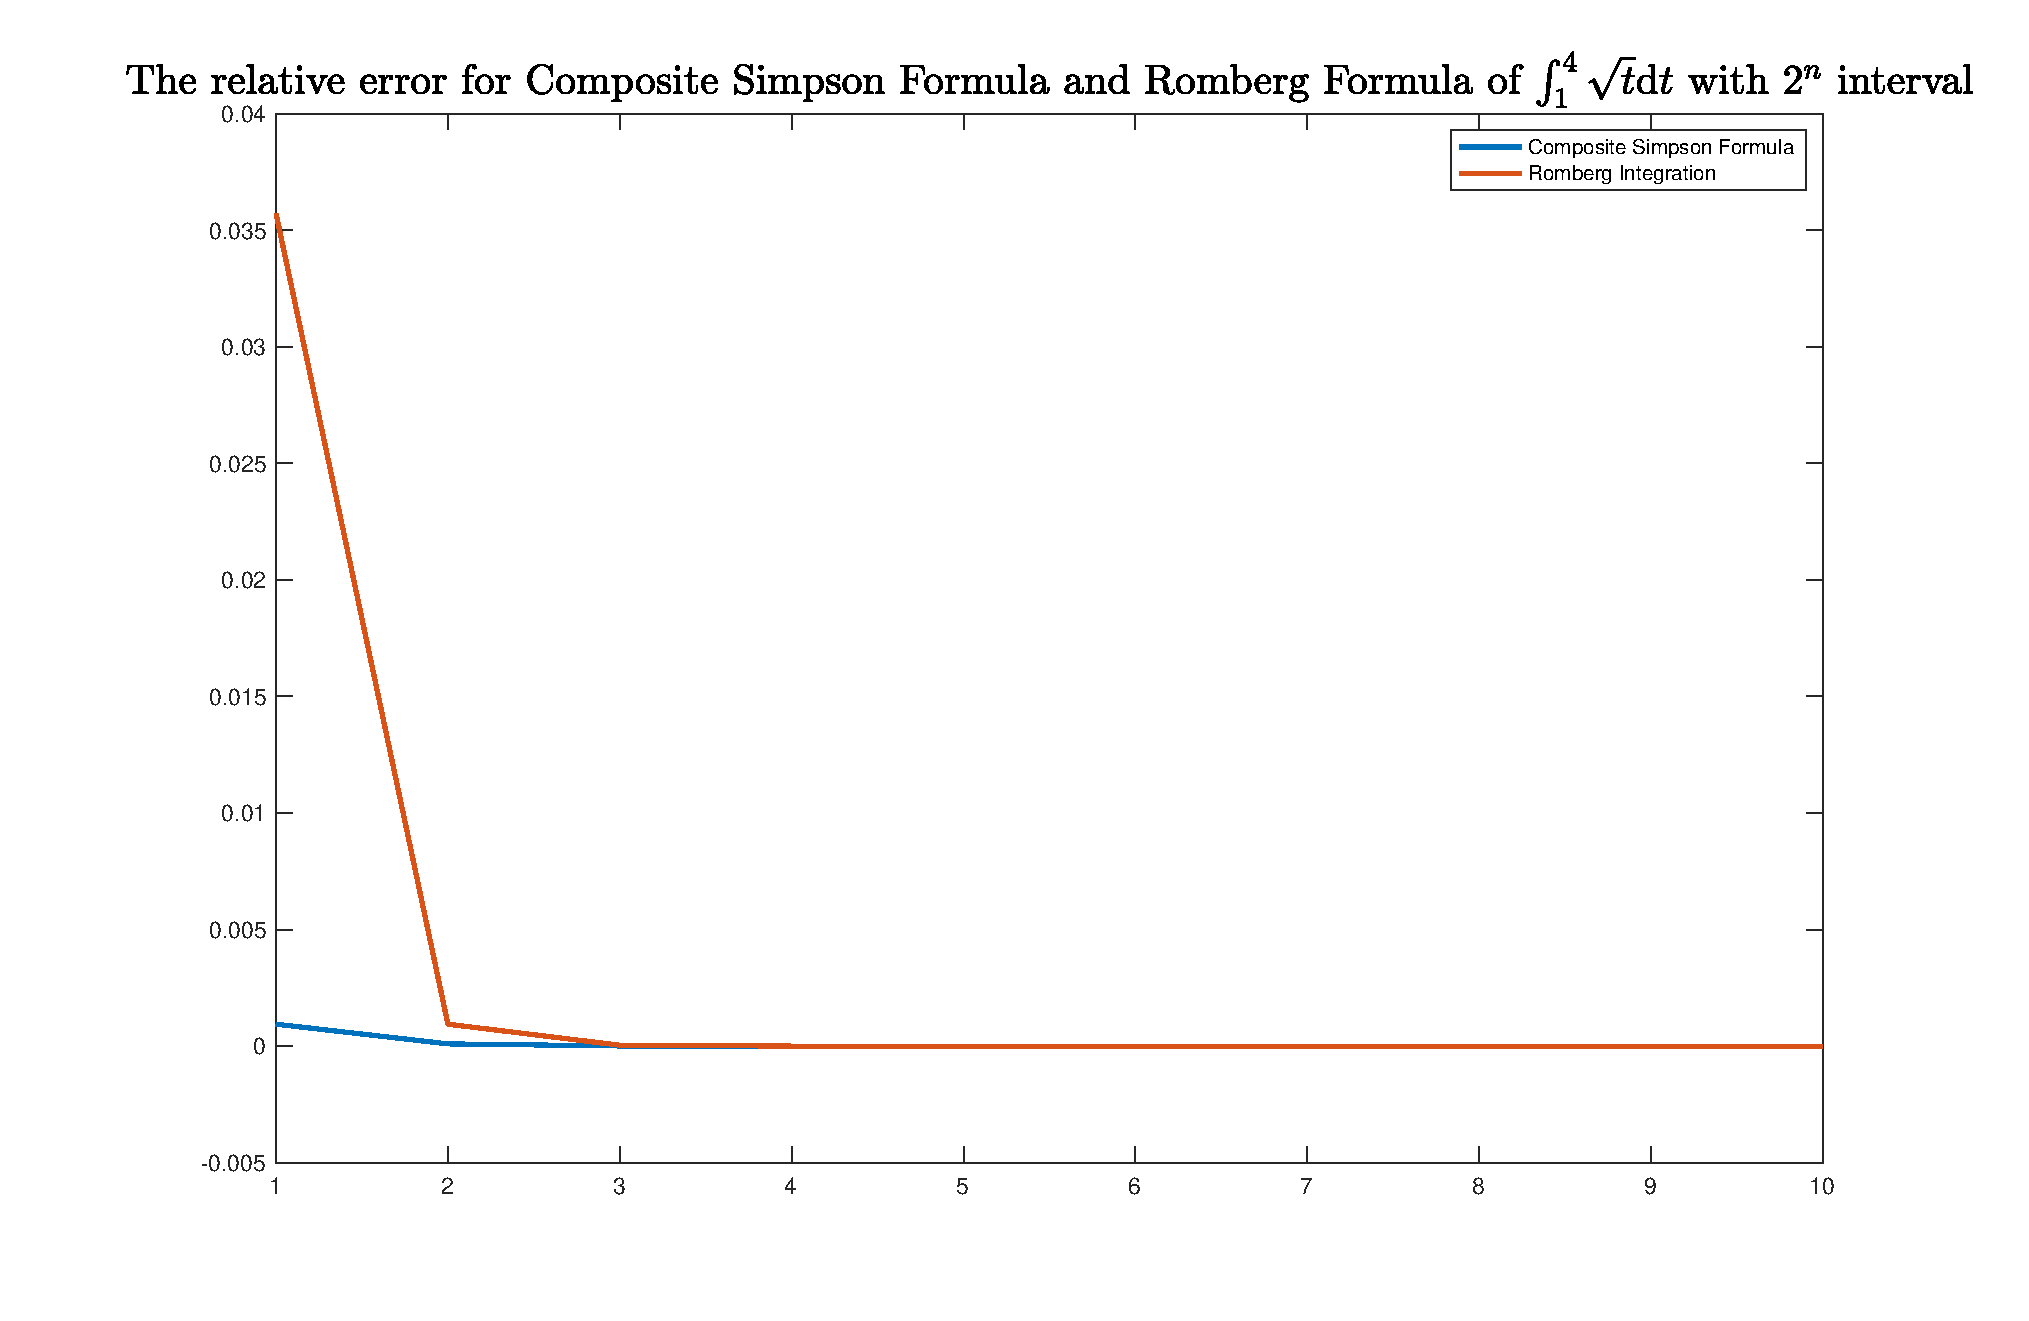
\includegraphics[width=15cm]{fig/Q3}
  \caption{The relative error for Composite Simpson Formula and Romberg Formula of $\int_1^4 \sqrt{t} \mathrm d t$ with $2^n$ interval} \label{Q3_graph}
\end{figure}


\end{solution}


